\begin{enumerate}
\item The five constraints are:

\begin{align*}
4/7x_1 - x_2  & \leq 4,& (1)  \\
2x_1  - x_2 & \geq 4,& (2)   \\
x_1+ x_2  & \leq 5, & (3) \\
x_2 &\leq 0, & (4)\\
x_1 &\geq 0. & (5)
\end{align*} 

\item Constraints (1) to (3), can be transformed into equality
  constraints by introducing slack variables $e_1, e_2, e_3 \geq 0$ as
  follows: 

\begin{align*}
4/7x_1 - x_2  + e_1 & = 4.  \\
2x_1  - x_2 - e_2 & = 4.   \\
x_1+ x_2  + e_3 & =5. 
\end{align*} 

For constraint (4) we use a change of variable. We define a new variable $ x'_2 \geq 0 $ as
\begin{equation*}
x'_2 = - x_2.
\end{equation*}

The non-negativity constraint on $ x'_2 $ ensures that $ x_2 \leq 0 $.

We replace $ x_2 $ with ($ -x'_2 $) in the objective function and all the constraints.
 
By putting  everything  together, the  problem in standard form is:
\[
\min  2 x_1 + x'_2
\]
subject to
\begin{align*}
 4/7x_1 + x'_2  + e_1 & = 4,  \\
2x_1  + x'_2 - e_2 & = 4, \\
x_1- x'_2 + e_3 & =5, \\
x_1, x'_2, e_1, e_2, e_3 &\geq 0.
\end{align*}

The number of equality constraints is $m=3$ and the number of decision variables is $n=5$.
The matrix  $A\in\mathbb{R}^{m\times n}$ and the vectors $b\in\mathbb{R}^{m}$ and $c\in\mathbb{R}^{n}$ are given by
\[
A = 
\begin{pmatrix}
4/7 & 1 & 1 & 0 & 0 \\
2 & 1 & 0 & -1 & 0 \\
1 & -1 & 0 & 0 & 1 
\end{pmatrix}, \qquad
b = \begin{pmatrix}
4 \\
4 \\
5 
\end{pmatrix}, \qquad
c = \begin{pmatrix}
2 \\
1 \\
0 \\
0 \\
0 
\end{pmatrix}.
\]

\item   Each basic solution is obtained by selecting $m=3$ variables out of $n=5$ to be in the basis.
The $n-m=2$ non basic variables equal  0.
There is a total of 10 possible selections of basic variables. We
detail the calculation of some of them:
\begin{itemize}
\item Basic solution with $x_1$, $x'_2$ and $x_3$ in the basis

 ($j_1=1$, $j_2=2$, $j_3=3$).
$$B=
\begin{pmatrix} 
4/7 & 1 & 1 \\
2 & 1 & 0\\
1 & -1 & 0
\end{pmatrix};
\quad
B^{-1}=
\begin{pmatrix} 
0 & 1/3 & 1/3 \\
0 & 1/3 & -2/3 \\
1 & -11/21 & 10/21
\end{pmatrix};
$$

$$
x_B = B^{-1}b=
\begin{pmatrix} 
3  \\
-2 \\
30/7  
\end{pmatrix};
\quad
x=
\begin{pmatrix} 
3  \\
-2 \\
30/7\\
0\\
0 
\end{pmatrix}.
$$ 
This basic solution is infeasible since $ B^{-1}b  \ngeq 0$. It corresponds to point B in Figure  \ref{fig:a19-bassol} 
which is the intersection of constraints (2) and (3).


\item Basic solution with $x_1$, $x'_2$ and $x_5$ in the basis 

($j_1=1$, $j_2=2$, $j_3=5$).
$$B=
\begin{pmatrix} 
4/7 & 1 & 0 \\
2 & 1 & 0\\
1 & -1 & 1
\end{pmatrix};
\quad
B^{-1}=
\begin{pmatrix} 
-7/10 & 7/10 & 0 \\
7/5 & -2/5 & 0 \\
21/10 & -11/10 & 1 
\end{pmatrix};
$$

$$
x_B = B^{-1}b=
\begin{pmatrix} 
0  \\
4 \\
9  
\end{pmatrix};
\quad
x=
\begin{pmatrix} 
0  \\
4 \\
0  \\
0\\
9 
\end{pmatrix}.
$$  
This basic solution is feasible as $ B^{-1}b  \geq 0$. It corresponds to vertex F in Figure  \ref{fig:a19-bassol}
which is the intersection of constraints (1) and (2).

\item  Basic solution with $x_1$, $x_3$ and $x_5$ in the basis 

($j_1=1$, $j_2=3$, $j_3=5$).
$$B=
\begin{pmatrix} 
4/7 & 1 & 0 \\
2 & 0 & 0 \\
1 & 0 & 1 
\end{pmatrix};
\quad
B^{-1}=
\begin{pmatrix} 
0 & 1/2 & 0 \\
1 & -2/7 & 0 \\
0 & -1/2 & 1 
\end{pmatrix};
$$

$$
x_B = B^{-1}b=
\begin{pmatrix} 
2  \\
20/7 \\
3  
\end{pmatrix};
\quad
x=
\begin{pmatrix} 
2  \\
0 \\
20/7\\
0\\
3 
\end{pmatrix}.
$$  
This basic solution is  feasible since $ B^{-1}b  \geq 0$. It corresponds to vertex D in Figure  \ref{fig:a19-bassol}
which is the intersection of constraints (2) and (4).
\end{itemize}


The following table gives all the basic solutions. Each basic solution is obtained by fixing
 $n-m=2$ non basic variables, which equal  0, and calculating the other variables using  
 $ x_B=  B^{-1} b$.

\begin{center}
%\resizebox{\textwidth}{6cm}{
	\begin{tabular}{|c||c|c||c|c|c|c|c||c||c|}
		\hline
		\text{Point} & $x_1$ & $x'_2$ & $e_1$ & $e_2$ & $e_3$ & Feasible? \\
		\hline
		A & 0 & - 5 &  9 & -9 &  0 & no \\
		B & 3 & -2 & 30/7 & 0 & 0  &  no \\
		C & 5 & 0 & 8/7 & 6  & 0 & yes \\
		D & 2 & 0 & 20/7 & 0 & 3  & yes \\
		E & 7 & 0 &  0 & 10 & -2  & no  \\
		F & 0 & 4 & 0 &	 0 &  9 & yes \\
		G & 63/11 & 8/11 & 0  & 90/11 & 0  & yes\\
		H & 0 & 0 & 4  & -4  &  5 & no\\
		\hline
	\end{tabular}
%	}
\end{center}


\begin{itemize}


\item In Figure  \ref{fig:a19-bassol}, the basic solutions are given with the same letters as on the table above: from A to H.
They correspond to the intersections of the constraints.


\begin{figure}[htb]
	\begin{center}
		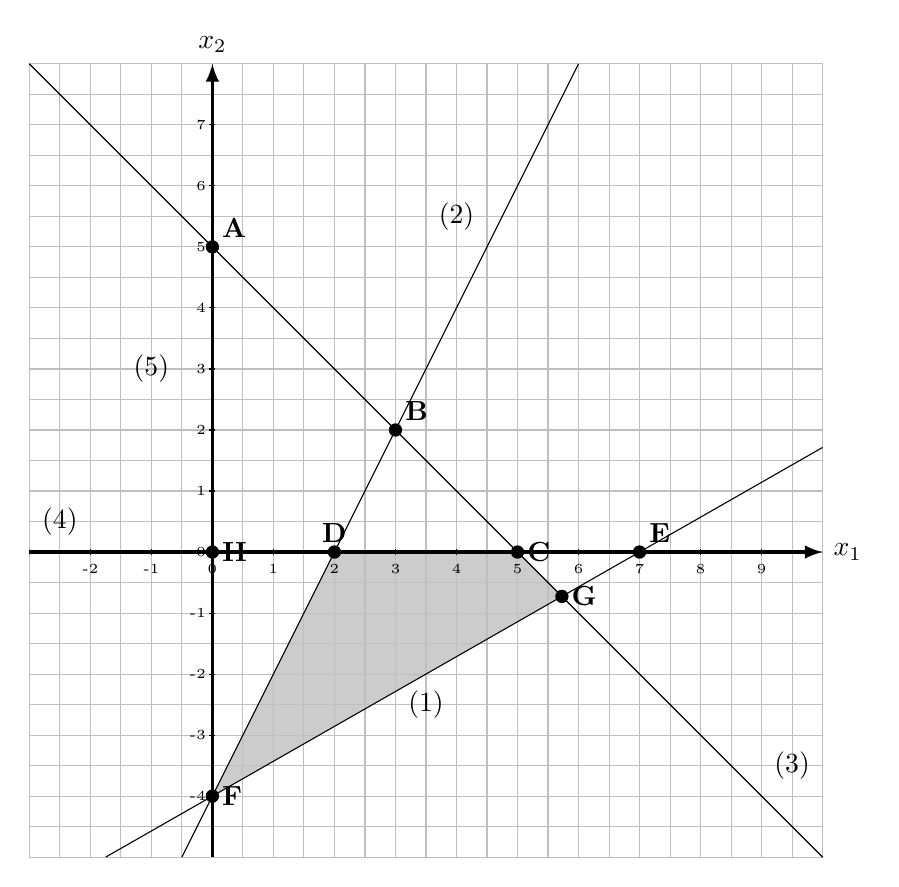
\begin{tikzpicture}[scale=0.775]
		\fill[gray,opacity=0.4] (0,-4) -- (63/11,-8/11) -- (5,0) -- (2,0)  --cycle; 
		\draw[gray!50, thin, step=0.5] (-3,-5) grid (10,8);
    	\draw[very thick,-latex] (-3,0) coordinate(x1) -- (10,0) coordinate(x2) node[right] {$x_1$};
    	\draw[very thick,-latex] (0,-5) coordinate(y1) -- (0,8) coordinate(y2) node[above] {$x_2$};
	    \foreach \x in {-2,...,9} \draw (\x,0.05) -- (\x,-0.05) node[below] {\tiny\x};
	    \foreach \y in {-4,...,7} \draw (-0.05,\y) -- (0.05,\y) node[left] {\tiny\y};
	
	
	    \draw (10,12/7)--(-7/4,-5);
	    \draw (-1/2,-5)--(6,8);
	    \draw (10,-5)--(-3,8);

		\node at (4, 5.5){(2)};
		\node at (3.5,-2.5){(1)};
		\node at (9.5, -3.5){(3)};
		\node at (-2.5,0.5){(4)};
	     \node at (-1,3){(5)};

	
		
		\draw [draw = black,fill=black] (0,5) circle (0.1) node[anchor=south west] {\textbf{A}};	
								
		\draw [draw = black,fill=black] (3,2) circle (0.1) node[anchor=south west] {\textbf{B}};
		
		\draw [draw = black,fill=black] (5,0) circle (0.1) node[anchor=west] {\textbf{C}};

		\draw [draw = black,fill=black] (2,0) circle (0.1) node[anchor=south] {\textbf{D}};
		
		\draw [draw = black,fill=black] (7,0) circle (0.1) node[anchor=south west] {\textbf{E}};
		
		\draw [draw = black,fill=black] (0,-4) circle (0.1) node[anchor=west] {\textbf{F}};
		
		\draw [draw = black,fill=black] (63/11,-8/11) circle (0.1) node[anchor=west] {\textbf{G}};
		
		\draw [draw = black,fill=black] (0,0) circle (0.1) node[anchor=west] {\textbf{H}};
		
		\end{tikzpicture}
		\caption{\label{fig:a19-bassol}Basic solutions}
	\end{center}
\end{figure}

\item A solution is feasible if it satisfies all the constraints of the problem. In order to calculate the basic solutions,
we used the formula  $ x_B= \nolinebreak  B^{-1}b$. 
The non negativity constraints still need to be satisfied. The feasible solutions satisfy  $$ x_1, x'_2, e_1, e_2, e_3  \geq  0.$$
Therefore, the feasible basic solutions correspond to the following points:
\begin{center}
D(2, 0), C(5, 0), G(63/11, -8/11) and F(0, -4).
\end{center}
They correspond to the vertices of the polyhedron.
\end{itemize}

\item $F(0,-4)$ corresponds to the solution $(x_1,x'_2,e_1,e_2,e_3
  )=(0,4,0,0,9)$. It is a degenerate basic feasible solution.  Indeed, three variables
  $x_1$, $e_1$ and $e_2$ are zero. This is strictly greater then $ n-m
  = 5-3 =2$. At the vertex
  $F(0,-4)$, three constraints are active: (1), (2) and
  (5). Activating two of them is sufficient to identify the
  vertex. The third one corresponds to a basic variables, that happens
  to be zero, as the corresponding constraint is active.
  This point corresponds to the three following
  bases:
 \[
B = 
\begin{pmatrix}
4/7 & 1  & 0  \\
2 & 1  & 0 \\
1 & -1 & 1 
\end{pmatrix}, \qquad
B= \begin{pmatrix}
1  & 1 & 0  \\
1  & 0 & 0  \\
-1  & 0 & 1  
\end{pmatrix}, \qquad
B = \begin{pmatrix}
1  & 0 & 0 \\
1  & -1 & 0 \\
-1  & 0 & 1 
\end{pmatrix}.
\]

\item When considering the problem in standard form, the point $(2, -2)$ corresponds to the
  point ($ x_1 $, $ x'_2 $, $ e_1 $, $ e_2 $, $ e_3 $) = $(2, 2, 6/7, 2, 5 )$. This is a feasible solution because all the constraints are
   satisfied. 

However,  in a basic solution at least $n$ constraints must be active.
 In standard form, $n=5$. There are $m=3$ equality constraints that are active. 
Therefore, at least two variables (the non basic variables) should be zero at a basic solution. 
It is not the case for the point $(2,- 2)$, so it is not a basic solution.

\item   Constraints (2) and (5) are active at point $F(0,-4)$ which corresponds to the solution  $(x_1,x'_2,e_1,e_2,e_3 )=(0,4,0,0,9)$ of the problem in standard form.
 
\begin{enumerate}
\item The corresponding basis matrix is 
\[
B = (x'_2,e_1, e_3)=
\begin{pmatrix}
1  & 1 & 0  \\
1  & 0 & 0  \\
-1  & 0 & 1  
\end{pmatrix}.
\]
\item The basic direction corresponding to the non basic variable $x_1$ is 
$$d_1 = P \begin{pmatrix} 
-B^{-1} A_1\\ 
1\\
0
 \end{pmatrix} 
= P \begin{pmatrix} 
-\begin{pmatrix} 
0 & 1  &0\\
1  & -1 & 0 \\
0 & 1 & 1 
\end{pmatrix} 
 \begin{pmatrix}
\frac{4}{7} \\
2 \\
1
\end{pmatrix} \\ 
1 \\
0 
\end{pmatrix} 
= P \begin{pmatrix}
 -2\\
\frac{10}{7} \\
- 3 \\ 
 1\\
 0
 \end{pmatrix} = 
  \begin{pmatrix}
 1\\
-2\\
 \frac{10}{7} \\ 
 0\\
 -3
 \end{pmatrix}.
 $$
 This direction is  feasible since for $x_1$, $e_1$ and $e_2$  the corresponding $d_{1i} \geq0 $.

 
 The basic direction corresponding to the non basic variable $e_2$ is 
$$d_2 = P \begin{pmatrix} 
-B^{-1} A_4\\ 
0\\
1
 \end{pmatrix} 
= P \begin{pmatrix} 
-\begin{pmatrix} 
0 & 1  &0\\
1  & -1 & 0 \\
0 & 1 & 1 
\end{pmatrix} 
 \begin{pmatrix}
0\\
-1 \\
0
\end{pmatrix} \\ 
0 \\
1 
\end{pmatrix} 
= P \begin{pmatrix}
1\\
-1\\
1 \\ 
 0\\
 1
 \end{pmatrix} = 
  \begin{pmatrix}
 0\\
1\\
-1\\ 
 1\\
 1
 \end{pmatrix}.
 $$
  
This direction is not feasible since $e_1 = 0$ and $d_{1 e1} = - 1 <0$.

\end{enumerate}


\end{enumerate}


